\documentclass[./main.tex]{subfiles}

\begin{document}

\chapter{Introduction}\label{chapter:introduction}

% Citation
"Only what is evolving is alive" \footnote{Pierre Kerner translation from french, original quote "N'est vivant que ce qui évolue"} this definition of life, like many others, is incomplete and we can probably found some corner case. This definition is based on the definition of evolution, we can try to define evolution of a thing, as the change on the thing to optimize her capability to conserve her self. To do that a thing need a memory.

In majority of actual know life the physical support of this memory was DNA for DeoxyriboNucleic Acid. DNA is a molecule compose by two strain, each strain was composed by phosphate backbone, along of these backbone we have sugar linked to a nucleic acid. We have four type on nucleic acid: Adenine (A), Thymine (T), Cytosine (C) and Guanine (G), Figure \ref{intro:fig:dna_rna_pres} show 3d structure of DNA.

The two strands of DNA are linked by their nucleic acid, with some rules in front of an A we will always have a T in front of a C we will always have a G and vice versa, a DNA strain was a complementary of the other. But we cannot add a new DNA base to each DNA strain at the same end, for some of chemical properties that we will not detail here, we say DNA was composed by two anti-parallel strain, by convention we represent DNA always in the same orientation.

In bioinformatics we generally represent a DNA strain by string in a four letter alphabet (A, C, T, G) the two property describe earlier allow us to reconstruct the composition of one strand from the other by apply complementary (replace A by T, T by A, C by G and G by C) and reverse order.

\begin{figure}[ht]
    \centering
    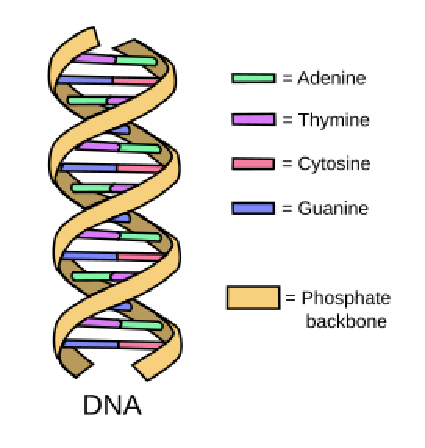
\includegraphics[]{introduction/images/DNA.pdf}
    \caption{Structure and composition of DNA Source: Wikipedia \protect\url{https://en.wikipedia.org/wiki/File:DNA_simple2.svg}}
    \label{intro:fig:dna_rna_pres}
\end{figure}

With mainy complexe and not details her, information contains in DNA was used to build essential molecules that keep the organism alive, reproduce it. This information is therefore the basis of the organism's functioning, if this information is destroyed or modified, the living organism will behave differently or died. So knowing and understanding the succession of DNA bases and therefore (but not the one) an effective entry point for analyzing many biological phenomena, disease, evolution,…

To read this information we have many biochemical techniques that we group under the term Sequencing techniques will allow us to read fractions of DNA fragments more or less long and with a variable error rate.

\section{Sequencing}

Sequencing technology evolve quickly since 1977\cite{sanger_sequencing}, even if it is an a posteriori reconstruction, three generations can be distinguished, based on reads property. In this section we didn't detail the biochemical methods we just focus on reads property and her impact on different bioinformatics task.

The two most important properties of a read are its size and error rate\. The longer of a read provide more information about his original sequence, which facilitate downstream analysis. If read contains many errors, the cost of downstream analysis increase and lost in precision and recall.

\begin{table}[ht]
    \centering
    \begin{tabular}{ll|rr|l}
Generation & Technology          & Read length (bd)                 & Error rate             & Source                          \\ \hline
Second     & ABI/Solid           & 75                               & Low ($\approx$ 2\%)    & \cite{seq_assembly_demystified} \\
Second     & Illumina/Solexa     & 100–150                          & Low (<2\%)             & \cite{seq_assembly_demystified} \\
Second     & IonTorrent          & $\approx$ 200                    & Medium ($\approx$ 4\%) & \cite{seq_assembly_demystified} \\
Second     & Roche/454           & 400–600                          & Medium ($\approx$ 4\%) & \cite{seq_assembly_demystified} \\
First      & Sanger              & $\approx$ 2 kb                   & Low ($\approx$ 2\%)    & \cite{seq_assembly_demystified} \\
Third      & Pacific Biosciences & $\approx$ 10 kb ($\max$ 100 kb)  & High ($\approx$ 18\%)  & \cite{seq_assembly_demystified} \cite{longread_dark_matter} \\
Third      & Oxford Nanopore     & $\approx$ 10 kb ($\max$ 1 mb)    & High ($\approx$ 12\%)  & \cite{longread_dark_matter} \cite{nanopore_read_accuracy} \\
    \end{tabular}
    \caption{This table present length of reads and error rate of main sequencing technology. Pacific Biosciences and Oxford Nanopore evolve quickly and this value change we have tried to be as up-to-date as possible but between two publications these values vary considerably.}
    \label{intro:tab:technology_property}
\end{table}

Sanger technique create large reads with very small error rate, but with a very low throughput and very expensive cost per base.
Second generation increase the throughput and reduce the cost per base, by reducing the length of the reads and increasing the probability of error ($\approx$ 1\%). This type of error are most of the time a substitution between two nucleotides, sequencer read \texttt{A} in place of a \texttt{T}.
The third generation has greatly increased the size of the reads but also the error rate while maintaining a descent throughput. Error in third generation are mostly insertion deletion, sequencer didn't read a part of sequence or generate random base not present in original sequence. Table \ref{intro:tab:technology_property} present read length and error rate on many sequencing technology.

DNA sequencing was very useful tools for many analysis, and in some cases is mandatory to be able to understand biological mechanisms. 
In important majority of case down stream analysis required:
\begin{itemize}
    \item mapping against a reference genome, found a subsequence in reference genome similar to the read
    \item found overlap between reads (or other set of reads), found similar sequence between reads 
\end{itemize}
 
\subsection{How to found similar region between sequence} 

\pim{Rajouté mapping}

Find overlap between reads are generally the bottleneck of many assembly pipeline.

This task have many link to plain text search. A simple description of this task could be, each reads are lines in a file, and for each line we will search in the file for lines that share suffixes or prefixes with our first line.

For first and second generation the main approach choose was the FM-index\cite{fm-index}. An FM-index is a compressed full-text sub string index based on idea we can use Burrows-Wheeler transform of text as a suffix array to perform an exact text search. First and second generation data didn't produce many error, so this method based on exact text search work well, we can cite \toolsname{SGA} as \OLC based second generation assembly pipeline use an FM-index to find overlap between reads. 

FM-index can be use for seed-and-extend technique, we search a short sub-sequence between reads with FM-index, if we have some common sub-sequence we can extend alignment between this seeds with \citeauthor{smith_waterman}\cite{smith_waterman} like algorithm.

This is a complete research field with many tools, and specificity of long-reads(length and high error rate) has relaunched this research field, \citeauthor{ovl_bench} produce an interesting review about some of third-generation overlap search in \cite{ovl_bench}. We details how two of them \mhap and \minimap works in section \ref{section:sota:canu} and \ref{section:sota:miniasm}.


\section{Assembly algorithm}

\pim{ajouter definition de contig unitig scaffold N50}

If you want study an organism, knowing the complete genome sequence is very useful for a lot of task like find the genes or the sequence variations across a population, understand how speciation affect genome. Yet, the best sequencing technologies still provide reads that are at least 2 orders of magnitude shorter than the genome. To understand the assembly problem, we provide a useful analogy which, to the best of our knowledge, has never been formulated before.

Imagine a crazy copyist monk. He is copying a book but he randomly chooses where he starts to copy, and he only copies small fragments of text at a time.
The copyist monks make errors, e.g. he would sometimes replaces a symbol by another one, would skip a symbol, or would add a random symbol. We respectively call these errors substitutions, deletions and insertions.
Now imagine that there are multiple such copyist monks.
They choose randomly where they begin to write. They can choose several times the same region of the book, never choose to copy a certain region, or more rarely copy another region. We refer by "coverage" the number of times a given chunk of the original book is copied. Coverage may significantly differ from one region to another.
In this analogy, the book is the genome of the organism we want to study, and the copyist monks are our sequencer. The fragments of text are reads, and the operation to rebuild the book is assembly.

The assembly task can be summary has a ordering problem we try to put the text fragments in the original book order.

To find the right order of book fragments, we can try to compare fragments and say that e.g. this fragment is the same of this one, or these two fragments share the same symbols at their extremities. When two fragment share a common sequence at their end of the fragment we say they overlap \ref{intro:fig:overlap:perfect}. Yet it possible for reads to share a common sequence just because alphabet have a fixed size, but the probability of this event decrease when the length of common sequence increase. Intuitively, this probability gets smaller as overlaps get longer. In perfect word, the only criteria to evaluate whether an overlap is "real" or not should be the length of the overlap, the only criteria to evaluate if an overlap is a true one should be his length. However the number of errors in each reads broke this paradigm and force us to build  yet an important factor do consider is that reads contain errors \ref{intro:fig:overlap:erroneous}.

To reconstruct the original sequence with short fragments (reads), finding the overlaps between these fragments constitutes the basis of many assembly algorithms.

\begin{figure}[ht]
    \centering
    \subfloat[ht][$R_1$ share 7 bases at its end with the beginning of $R_2$, without any error]{
        \subfile{introduction/tikz/perfect_overlap.tex}
        \label{intro:fig:overlap:perfect}
    }
    \subfloat[ht][$R_1$ share 5 bases at its end with $R_3$, with one substitution and one deletion]{
        \subfile{introduction/tikz/erroneous_overlap.tex}
        \label{intro:fig:overlap:erroneous}
    }
    \caption{When reads didn't contains error all overlap look like (a) but}
    \label{intro:fig:overlap}
\end{figure}

\pim{Ajouter définition contig unitig}

\subsection{\textit{Greedy} assembly algorithm}

\pim{quand sa a utilisation pourquoi cité au moins un outils}

The \textbf{Greedy} assembly algorithm are the first type of assembly tools, used on Sanger data. Algorithm \ref{intro:algo:greedy} present global idea how \textbf{Greedy} algorithm work.

The BEST\_OVERLAP function is the main part of algorithm the best overlap is the larger one or the overlap with less error, each algorithm have her own choose method.

\begin{algorithm}[ht]
    \caption{A greedy assembly}
    \begin{algorithmic}[1]
    \Function{greedy}{reads}\Comment{reads is a set of read}
        \State choose r1 in reads
        \State sequence $\leftarrow$ r1
        \While{r2 $\leftarrow$ \Call{best\_overlap}{r1}}\Comment{\Call{best\_overlap}{\null} is a function for r1 they get read r2 the best overlap for read r1 in reads}
            \State \Call{concatenate}{sequence, r2}
            \State \Call{drop}{r1, reads}
            \State r1 $\leftarrow$ r2
        \EndWhile
    \EndFunction
    \end{algorithmic}
    \label{intro:algo:greedy}
\end{algorithm}

Moreover \textbf{Greedy} algorithm, by focusing on the local problem, weach overlap is the best one for this read, can't manage repetition. Genome contains many repetition, like a book some word are reused or complete part of sentence can be present multiple time.

Figure \ref{intro:fig:greedy:repetition} present a case where reads $R_0$ $R_1$ and $R_2$ contains a repetition. $R_0$ have two possible overlap if overlap with $R_1$ is choose the assembly sequence match with the green path, if overlap with $R_2$ is choose the assembly sequence match with the red path. We can't know weach path is the good one and we didn't see the repetition. So assembly tools based on \textbf{Greedy} algorithm can produce many misassembly. 

\begin{figure}[ht]
    \centering 
    \subfile{introduction/tikz/repetition.tex}
    \caption{Each black box are a read, the grey box mark the position of a repetition. The begin of $R_1$ and $R_2$ are in repetition they share same begin but didn't match at her end. This repetition create a ambiguity in assembly.}
    \label{intro:fig:greedy:repetition}
\end{figure}

\subsection{Overlap Graph Consensus}

\pim{quand sa a utilisation pourquoi cité au moins un outils}

An alternative of \textbf{Greedy} approach was Overlap Graph Consensus (\OLC). This approch was based on a graph where read was a node and we build a edge between node if reads share an overlap. Figure \ref{intro:fig:olc:graph}, present the \OLC corresponding to ovelap present in \ref{intro:fig:greedy:repetition}.

We can see this graph like an ordering of piece of book provide by crazy copyist monk, an edge indicate this piece of text was before this piece of text in the original book.

The repetition create a fork in \OLC, a node with two successor, it's easy to detect this case in graph and stop assembly. The result of assembly of this graph was 3 sequences with white node, green node and red node. The assembly was more fragmented than \textit{Greedy} algorithm but the assembly didn't contains misassembly.

\begin{figure}[ht]
    \centering 
    \subfile{introduction/tikz/overlap_graph.tex}
    \caption{Each node are a read and an edge was build between two read if they share an overlap.}
    \label{intro:fig:olc:graph}
\end{figure}

By analyzing the graph we will be able to detect the paths with out branching node in the graph and reconstruct the corresponding sequence by merging the sequences present in the graph.

\pim{parlé des défauts long et couteux en mémoire}

\subsection{DeBruijn Graph}

A main trouble of \OLC strategy was the cost to find overlap between reads. In \citeauthor{eulerian_approach} in \cite{eulerian_approach} propose a new approch to solve assembly problem, without search of overlap between reads.

This approach was based on DeBruijn Graph (or \DBG), for an alphabet with $n$ symbol a \DBG represent each word of length $k$ as node and build a directed edges if node share $k - 1$ symbol at extremity, for example in Figure \ref{intro:fig:dbg:graph} node \texttt{ATCG} and \texttt{TCGG} share \texttt{TCG}. A word of length $k$ was called a \kmer.

In assembly problem $n = 4$ (${A, C, T, G}$), and we can choose a value of k between 1 and the length of read. In practice this size is often smaller than the size of a reads is the choice of the right values of k, depending on the use that we will have of the \DBG graph could be the subject of a completed thesis.

To build the \DBG we choose a value of $k$ and we add all \kmer present in reads in the \DBG. The \DBG used in assembly contains only \kmer present in dataset not all possible \kmer, and edge can be only edge present in dataset or all possible edges.

\begin{figure}[ht]
    \center
    \subfile{introduction/tikz/debruijn_graph.tex}
    \caption{We have a dataset of 4 reads with length equal to 7, we choose a value equal to 4, kmer was present under each read. A \DBG build from this kmer set was present under kmer, each node was a kmer and if a word share $k - 1$ symbol at is end with $k - 1$ symbol at begin of another node we build a directed edge. This \DBG contains cycle this cycle probably match with a repetition in original sequence}
    \label{intro:fig:dbg:graph}
\end{figure}

Like \OLC we can detect repetition by inspect the number of successor of a node Figure \ref{intro:fig:dbg:graph} present a \DBG with a repetition. After build the \DBG we can follow the simple path to rebuild the original sequence.

With \DBG strategy we didn't compute overlap between reads, but the length of word in graph was shorter. And all repetition with a size upper than $k$ create cycle in the graph and fragment the assembly.

Moreover the overlap between word in \DBG must exact (without error) and with a fixed length ($k - 1$), these two constraints are particularly problematic when the reads contain a lot of error or when the coverage of the region is low.

\subsection{Graph cleaning}

Graph structure was usefull to have complete view on all information provide by reads, but having too much information can create problems, slow down the assembly tools and increase their costs in memory or at worst lead to misassembly or to unnecessary fragmentation of the assembly.

\subsubsection{Transitive edge}

In Figure \ref{intro:fig:olc:graph} you can notice edge from $R_1$ to read $R_3$, this overlap was exact we can found an overlap between $R_1$ and $R_3$. But this edge didn't provides a new information we know $R_1$ is before $R_3$, this edge was call a transitive edge. More formally we can define a transitive edge, in a directed graph if we have this set of edge $(a, b)$ $(b, c)$ and $(a, c)$ the edge $(a, c)$ is transitive.

\citeauthor{string_graph} propose in \cite{string_graph} another assembly graph the \textbf{string graph} is an overlap graph without transitive edge. The string graph by reduce the number of edge in graph simplify traversing of the graph and memory impact of this one.

With string graph we just need follow simple path (path were all nodes have just one successor), to build assembly without misassembly.

\subsubsection{Contained reads}

In third generation technology, the crazy copyist monk provide fragment with different size and choose the begin of fragment randomly, so it's possible to have a read is contained in another one. All information (kmer or overlap with other reads) in contained reads was present in the container read for assembly task we can remove contained read, and save memory and time.

\subsubsection{Bubble and tips}

\OLC and \DBG was based on graph, the meaning of nodes and edges are different in this type of graph. But we can found same structure in them, bubbles and tips.

Figure \ref{intro:fig:cleaning}

\begin{figure}[ht]
    \subfloat[][A example of tips in an assembly graph, the tips node wase represent in read, green, blue and black line underline different possible assembly scenario]{
        \subfile{introduction/tikz/cleaning_tips.tex}
        \label{intro:fig:cleaning:tips}
    }
    \subfloat[][A example of bubble in an assembly graph, each path was colored in different color. The length of each path can be different and we can have more than two path in bubble]{
        \subfile{introduction/tikz/cleaning_bubble.tex}
        \label{intro:fig:cleaning:bubble}
    }
    \caption{}
    \label{intro:fig:cleaning}
\end{figure}

A tips in an assembly graph is a node with only one edge, a tips can be create by many thing, trouble during DNA extraction, DNA duplication, sequencer create an artifact, a read with to many error ….

As we can see in Figure \ref{intro:fig:cleaning:tips} a tips can create a branching node in middle of simple path, if we keep this tips generally assembly create two contigs one before tips and one after tips (green and blue assembly scenario). If we remove this tips we can run the black scenario.

Its easy to detect and remove tips in graph, in many assembly tools tips are considered as errors and are removed.

We can define a bubble as a set of subpath in graph with same parent and same children, Figure \ref{intro:fig:cleaning:bubble} present an example with two path with same length. The bubble can be create by repetition or heterozygotie one or more version of this sequence contains a substitution or more complex mutation.

If bubble are large it can be harder to detect, with small bubble one version of the bubble are kept the choose of the version can be based on random choice or on coverage or other magic tricks.

\section{Why people use long reads}

The length of read have a huge impact on assembly, before third generation sequencing the maximum length of read is lower than 2 kb (for Sanger read) or a majority of repetition in genome are larger than this length. \citeauthor{one_chromosome_one_contig} in \cite{one_chromosome_one_contig} indicate a theoretical length of read to obtain a perfect genome assembly for bacteria, read need to be upper than 7 kb, this limit not work in all practical case. If read are longer than repetition read can have a sufficient length before repetition cover all repetition and sufficient length after repetition we can solve the repetition see Figure \ref{intro:fig:whylongreads}.

\begin{figure}[ht]
    \centering
    \subfile{introduction/tikz/whyrepetition.tex}
    \caption{We have a part of assembly graph (\OLC or \DBG), node \texttt{R} represent a repetition node \texttt{A}, \texttt{B}, \texttt{C}, \texttt{D} represent basic sequence. Red, purple, green and blue line represent reads. Red read was larger than repetition and span over it and indicate $A_1 \rightarrow A_2 \rightarrow R \rightarrow C_1 \rightarrow C_2$ was a good path, with out this read we can solve this repetition.}
    \label{intro:fig:whylongreads}
\end{figure}

Third generation read aren't larger than all repetition but larger than many repetition and they help to produce better genome assembly. We can take as an example the gorilla genome where N50 was increase by a factor 1000 with an pacbio assembly with Falcon \cite{gorilla_genome}.


\pim{bien faire passé le message que les reads de troisième génération c'est cool}

\section{Assembly Trouble}

Third generation come with her own trouble, mainly a different error profile many insertion deletion low substitution than previous technology, reads with a different length, this difference required to devllop new tools for this type of data.

During my thesis I focus only on trouble before assembly step and after assembly of thrid generation reads.

\pim{Indique pour chaque problème si on y répond comment et dans qu'elle section}

\subsection{Data management}

Sequencing generate more and more data, and long-read sequencing technology work how to increase the throughout of sequencer. Tools around long-read assembly generate more data (overlap, assembly graph, contigs, hétérozygotie), and many times all this data isn't useful for a specific downstream analysis.



Can we filter overlapping information with a positive (or not very bad) impact on assembly result, to increase speed of assembly and the impact of assembly step on disk space ?

We present our solution of this problem \fpa in section \ref{section:preassembly:yacrd_fpa}, overlaper output can by pipe directly in \fpa (for Filter Pairwise Alignment), \fpa can filter overlap with some filter, length of read, length of overlap, type of overlap, read name. Some simple \fpa filter reduce the computation time of assembly without effect (or a small positif effect) on assembly, read section \ref{section:preassembly:yacrd_fpa} for more details on this tools.

\subsection{Correction work but not good enough}

The sequencing depth is not homogeneous and if for a given region this depth is not sufficient for the corrector, it will be less effective but it could still reduce the sequencing depth by eliminating reads or part of reads. To solve this problem it is necessary either to work without correction or to return to the raw reads to find the lost connection.

At the best of our knowledge the only one reads correctors they try to keept the hetrozygotie during correction is falcon \cite{falcon}, the other didn't try to keep this information. Or heterozygotie are very use full to understand genetic diversity in population or some genetic disease.
Moreover if you genome contain some almost repetion (two instance of same text with some mutation), the correction maybe can't distinguish the mutation between this two instance to sequencing error and correct the two instance of the almost repetition to the same sequence, so correction can create a repetition that cannot be resolved where there were we have two solvable almost repetitions 

\begin{table}[ht]
    \centering
    \begin{tabular}{c|c}
         &  \\
         & 
    \end{tabular}
    \caption{Time and memory usage of three self corrected long reads, compare to two most popular long reads assembly. For \canu we messure separatly the correction and the assembly module, on long reads dataset XXXXXX.}
    \label{intro:tab:correctionvsassemblytime}
\end{table}

Table \ref{intro:tab:correctionvsassemblytime} we can see the correction two orders of magnitude more time to be started and four orders of magnitude more memory. Moreover, as the table \ref{intro:tab:assembleandcorrect} shows, it would seem that assembling the raw reads and then correcting the contigs would be more interesting than correcting the reads and then assembling them.

\begin{table}[]
    \centering
    \begin{tabular}{c|c}
         &  \\
         & 
    \end{tabular}
    \caption{}
    \label{intro:tab:assembleandcorrect}
\end{table}

Specific long-error profile with a majority of indel create some difficulty to found gene in long-reads assembly (corrected by short-reads or only by long-reads), by create frame shift \cite{blog_post_gene_detection}. A very low error rate in genome assembly with long-reads can be archived but only by assembly tools expert.

Correction of reads before assembly can generate some trouble in assembly and remove some important information. But long-reads still contains very low quality region \cite{blog_post_error_repartition} this region can lead to a fragmented assembly \cite{long_read_assembler_comparison}. 

To found and remove this very low quality region and read we create \yacrd, \yacrd use self overlapping information to compute a coverage curve and identify region with low coverage. We suppose this low coverage region is region with low quality, read section \ref{section:preassembly:yacrd_fpa} for more details on this tools.

\subsection{Trouble with heuristic algorithm}

\pim{parler de https://github.com/rrwick/Long-read-assembler-comparison}
\pim{cité les papier de l'intro de knot sur l'annalyse d'assemblage}

Assembly tools perform a great job, but they can't explore all space.
Due to memory constraint and cpu usage you can't build and store all overlap.
Due to theoretical limit, how many of base need to be share between to read to create an overlap how many error we can accept in this overlap.

Assembly tools need use heuristic algorithm, solve assembly trouble in this constraint, in majority of case this heuristic perform a very good work, but in some case we need perform a more complex analysis.

\citeauthor{long_read_assembler_comparison} in \cite{long_read_assembler_comparison} perform a comparison of five assembly tools on real data and simulated data bacterial data set. Some trouble in long-reads was simulated to stress assembly tools:
\begin{itemize}
    \item adaptator length, sequencing require add short sequence before reads, remove this adaptator in long-read sequencing technology aren't trivial
    \item chimeric read, during DNA extraction and fragmentation two fragment come from different region an can lead to assembly fragmentation
    \item glitch level, long-read error aren't uniformly distributed along the reads and sometimes sequencer create a region with only random sequence. A more important the glitch level indicate the bigger the glitch will be and the more frequently it will happen
    \item random junk read, some read are just a string of random character
    \item read depth, correspond to genome coverage
    \item read identity, percent of error insertion, deletion, substitution 
    \item read length, length of read 
\end{itemize}

\begin{figure}
    \centering
    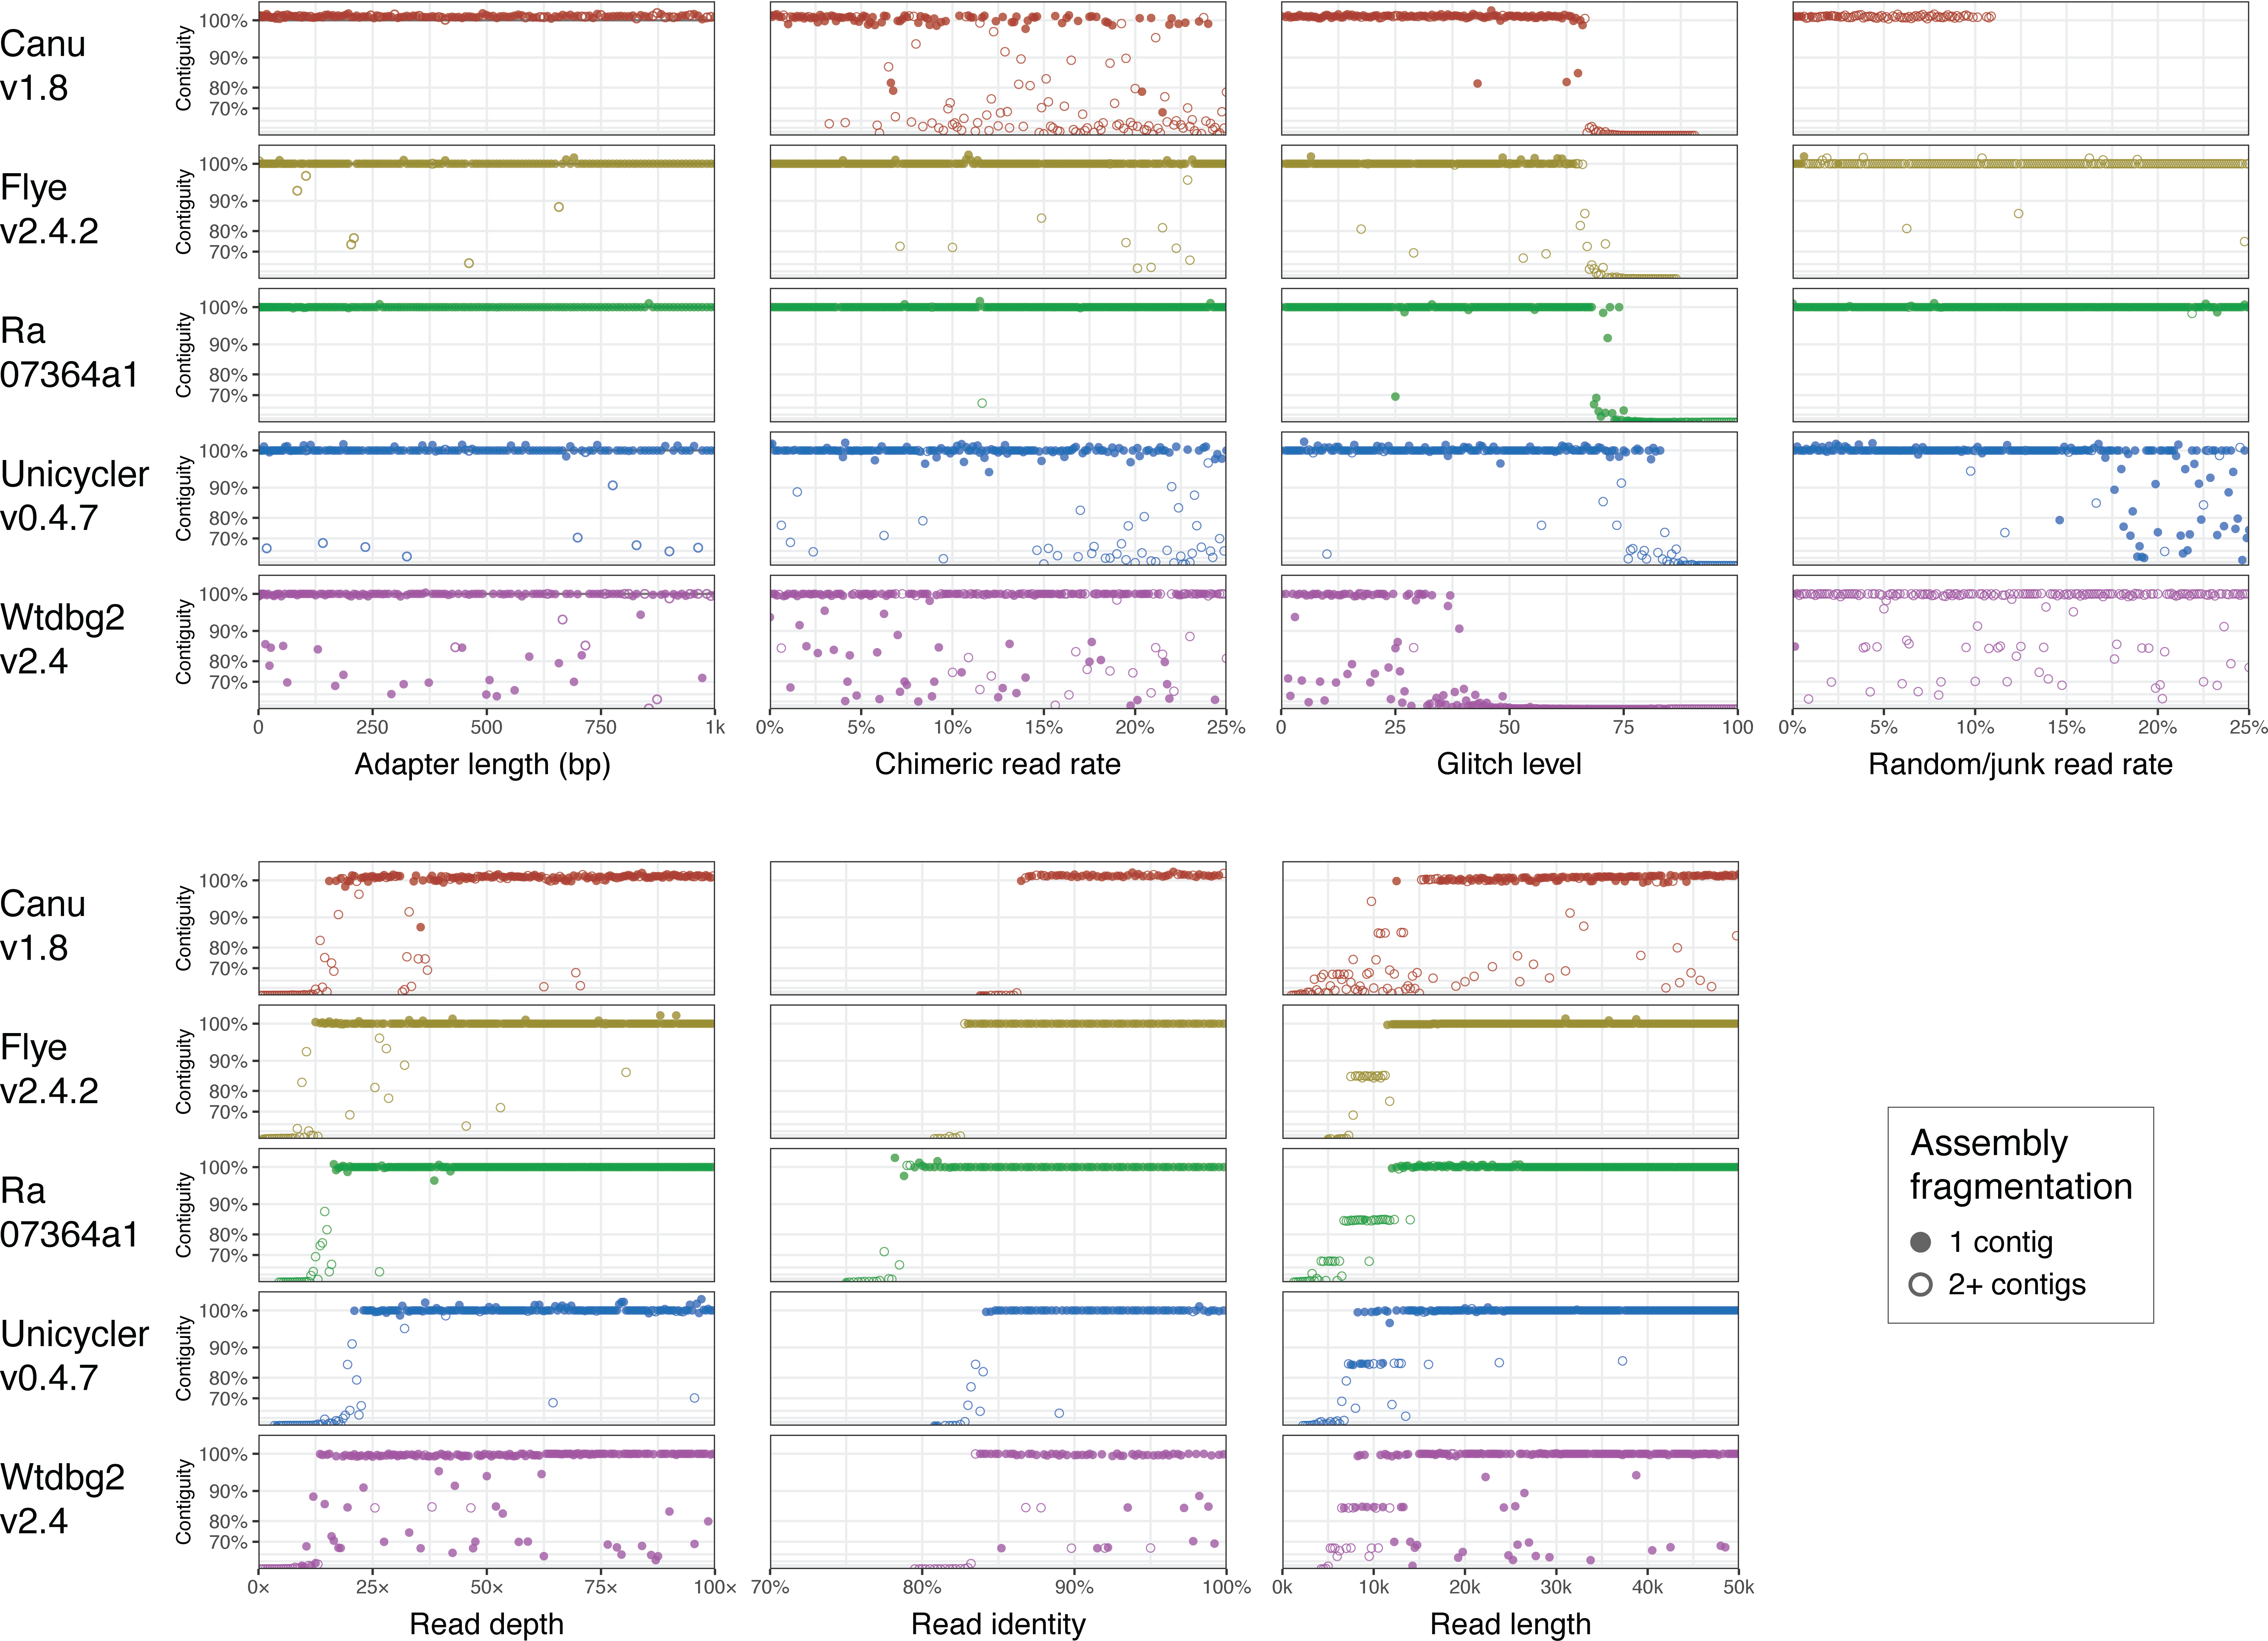
\includegraphics[width=\textwidth]{introduction/images/rrwick_bench.png}
    \caption{Effect of different reads property on assembly contiguity (number of contigs expect and map correctly on reference genome), of five assembly tools, \toolsname{Unicycler} was an hybrid assembler (use second and thrid generation read), \canu was a long-read assembly pipeline they perform a self correction before construct assembly with a special \OLC graph (more detail in Section \ref{section:sota:canu}), \toolsname{Ra} perform a basic string graph assembly on raw reads with a correction of contigs after assembly (more detail in Section \ref{section:sota:miniasm}), \wtdbg and \toolsname{Flye} use a \DBG like approach to perform assembly on raw reads (more detail in Section \ref{section:sota:wtdbg})}
    \label{intro:fig:rrwick_bench}
\end{figure}

This study focus on contiguity of assembly, if the number of contig match with the expected number of contig and if this contigs map against the reference. All assembly perform a good assembly when:
\begin{itemize}
    \item reads length are upper than 10k and lower than 20k, this length was reach by long-read sequencing techonology but requests a particular attention be focused on the risk of DNA fragmentation
    \item read identity need to be upper than 85\% except
    \item a minimal coverage is around 20x, but this study didn't analyze the error rate of assembly we can suspect an high error rate in assembled contigs
    \item Chimeric read have an important impact on assembly contiguity but at level generally not observe in real data
\end{itemize}

We can observe an important variability of result (in \canu, \wtdbg and \toolsname{Unicycler}), an assembly can failled for many reason a chimeric read in a repetition, a drop of coverage, a missing overlap, or a not wheel chosen set of parameter.

We notice some times an overlapping tools mis an overlap found by another on and we notice an important space of progress in overlapping tools on real data \cite{ovl_bench}. In section \ref{section:preassembly:ovl_consensus} we present a blog post and a poster, about difference between overlapping tools result and some preliminary result of an overlapping tools consensus.

Analysis and understanding of data produce by assembly tools, help to understand and sometimes solve assembly trouble, coverage gap produce by correction, refund link between contigs, tag contigs they probably share a repetition. We create \knot a tools to simplify analysis of assembly tools result and help user to make choice for improve assembly quality. We present this work in section \ref{section:postassembly:knot}..

\onlyinsubfile{
\bibliographystyle{plainnat}
\bibliography{introduction,state_of_the_art}
\addcontentsline{toc}{chapter}{Bibliography}
}

\end{document}